\documentclass[a4paper, 11pt, titlepage]{jsarticle}
\usepackage{listings}
\usepackage[dvipdfm]{graphicx}

\title {知能情報実験1 : レポート課題4}
\author{205713B  朝比奈 太郎}
\date{\today }

\begin{document}
\maketitle
\tableofcontents
\clearpage

\section{目的}
Python科学ライブラリNumpyのadd関数を使用した場合とPythonの標準ライブラリの加算演算子(+)をを使用して要素ごとに加算した場合の処理時間を比較し、それぞれの使用用途を的確にするため。
また、加算演算子があるのにもかかわらずPython科学ライブラリNumpyのadd関数が存在しているということは、add関数の方が計算スピードにおいて優秀であるという自分の考えを確かめるため。
\section{方法}
\subsection{Numpyのadd関数を使用する場合}
importしたtimeのt0 = time.time()をadd関数の前の行に入れ、add関数の後ろの行にt1 = time.time()を入れ、t1 -  t0でadd関数における行列演算にかかった時間を求める。
\subsection{加算演算子(+)を使用する場合}
importしたtimeのt0 = time.time()を加算演算子を行うfor文の前の行に入れ、加算演算子を行うfor文を抜けた次の行にt1 = time.time()を入れ、t1 -  t0で加算演算子(+)における行列演算にかかった時間を求める。

\section{結果}
\subsection{(1,N)の1次元行列}
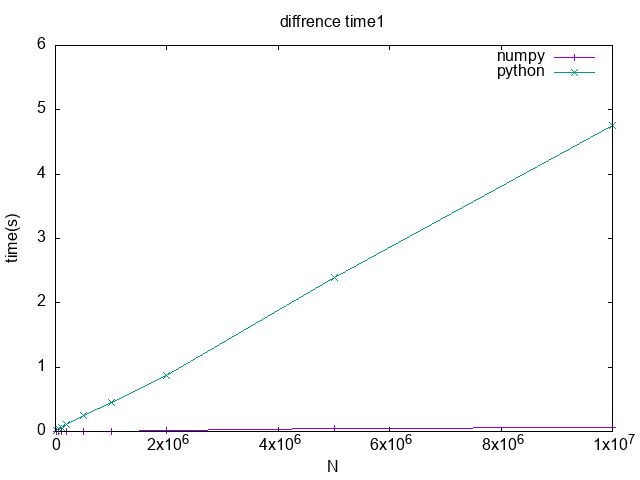
\includegraphics[width=15cm]{data1.png}\\
\\上図(diffrence time1)は,x軸がN, y軸がtime(s)となっている。
numpy,pythonを指すグラフは共に1次関数となっており、pythonのグラフの傾きがnumpyのグラフの傾きよりも大きいことから、numoy(add関数)よりも、python(加算演算子)の方が計算にかかる時間が長いといえる。従って、1次元行列の計算をする際にはPython科学ライブラリNumpyのadd関数を使用する方が計算速度が早くて良いと言える。
\clearpage
\subsection{(M,M)の2次元行列}
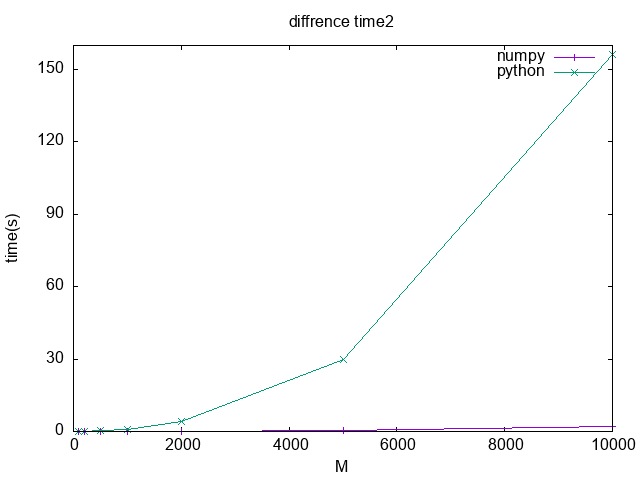
\includegraphics[width=15cm]{data2.png}
\\上図(diffrence time2)は,x軸がN, y軸がtime(s)となっている。
numpyのグラフは、diffrence time1と同様に1次関数になっているが、pythonのグラフは、2次関数のような形をとっている。Mが0から1000までの間はnumpyのグラフとpythonのグラフのtime(s)に関する値に目視できるほどの差はないが、Mが1000付近になるとnumpyとpythonのグラフのtime(s)をとる値に差が出始め、それ以降pythonのグラフがnumpyのグラフにtime(s)において大きく差が出る。
従って、正方行列の計算をする際にはMが1000未満の際は加算演算子(+)とNumpyのad関数のどちらを用いても良いが、それ以上になる際には、Python科学ライブラリNumpyのadd関数を使用する方が計算速度が早くて良いと言える。
\clearpage
\subsection{ソースコード}
\lstinputlisting[language=Python, numbers=left, breaklines=true, basicstyle=\ttfamily\footnotesize, frame=single, caption=ソースコード, 
label=pg:sample]{205713B.py}

\section{考察}
上図(diffrence time1,diffrenve time2)より、計算する量(N,M)が大きくなるにつれadd関数が加算演算子より早く計算できることがわかった。計算する量が少なくても、add関数と加算演算子ではかすかにadd関数の方が計算スピードが早いので、NumPyを利用するべきだと言える。
\begin{thebibliography}{99}
\bibitem{kunita} 國田 樹, 2021\_StuLab1\_理工系のレポート作成技術 , 2021/05/29.
\bibitem{Tex} Latex入門/図表, https://texwiki.texjp.org/?LaTeX, 2021/05/29
\end{thebibliography}
\end{document}